\documentclass{article}%
\usepackage[T1]{fontenc}%
\usepackage[utf8]{inputenc}%
\usepackage{lmodern}%
\usepackage{textcomp}%
\usepackage{lastpage}%
\usepackage[head=40pt,margin=0.5in,bottom=0.6in]{geometry}%
\usepackage{graphicx}%
%
\title{\textbf{Reportaron hallazgo de siete cadáveres en la mina de Tumeremo}}%
\author{El Nacional Web}%
\date{17/10/2018}%
%
\begin{document}%
\normalsize%
\maketitle%
\textbf{URL: }%
http://www.el{-}nacional.com/noticias/sucesos/reportaron{-}hallazgo{-}siete{-}cadaveres{-}mina{-}tumeremo\_256086\newline%
%
\textbf{Periodico: }%
EN, %
ID: %
256086, %
Seccion: %
Sucesos\newline%
%
\textbf{Palabras Claves: }%
Sucesos, Bolívar, Sociedad\newline%
%
\textbf{Derecho: }%
3.2, %
Otros Derechos: %
1.10, %
Sub Derechos: %
3.2.1, 1.10.1\newline%
%
\textbf{EP: }%
NO\newline%
\newline%
%
\textbf{\textit{Familiares de los fallecidos protestaron para exigir la entrega de los cuerpos}}%
\newline%
\newline%
%
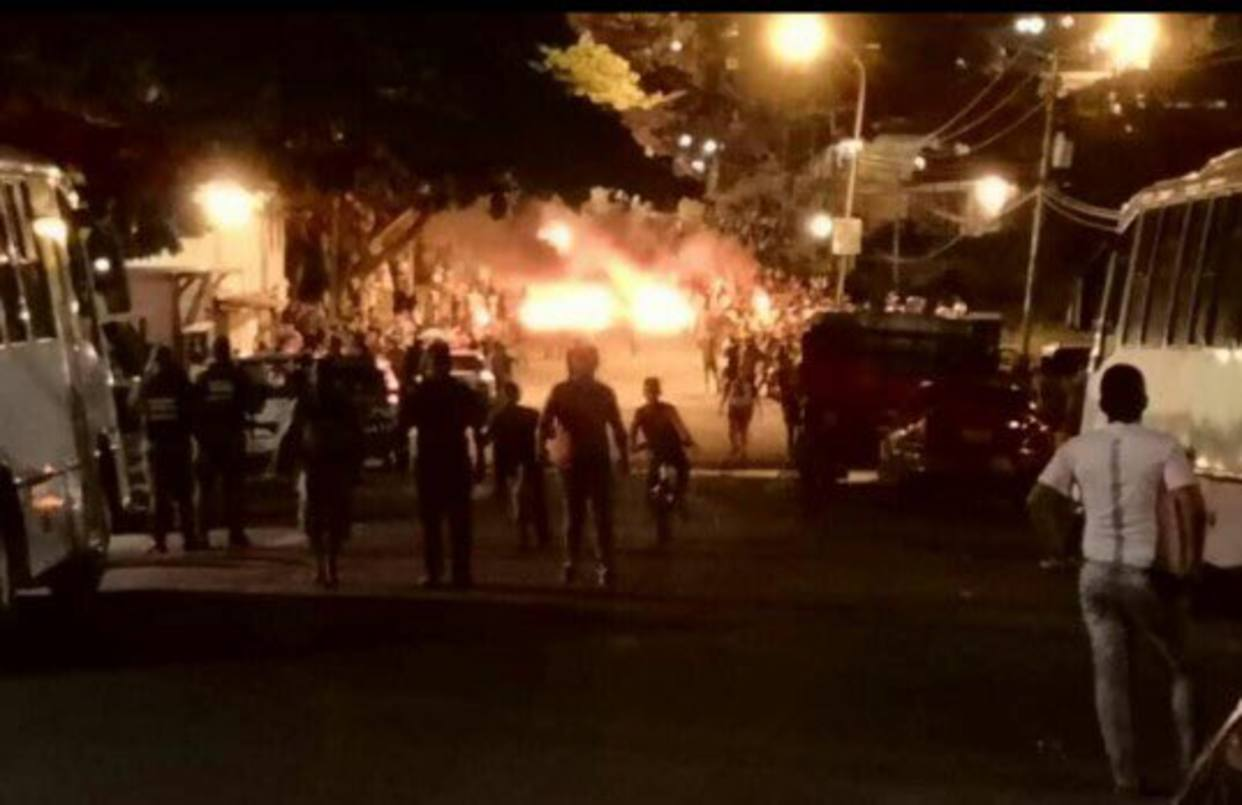
\includegraphics[width=300px]{147.jpg}%
\newline%
%
Américo de Grazia, diputado a la Asamblea Nacional por el estado Bolívar, informó este martes que fueron encontrados siete cadáveres en la mina El Candado de Tumeremo. El hallazgo lo realizaron funcionarios de las comisiones delegadas para el caso.%
\newline%
%
“Siendo las 7:40 pm de la noche en Tumeremo confirman el ingreso al Fuerte Militar Tarabay de 7 cadáveres en avanzado estado de descomposición, 3 mujeres y 4 hombres, aún no identificados”, escribió el parlamentario en Twitter.%
\newline%
%
A su vez, indicó que familiares de los fallecidos protestaron en la Troncal 10, a la altura del terminal de pasajeros, en rechazo a lo ocurrido con los mineros de la entidad, además exigieron que se les haga entrega de los cuerpos de los difuntos.%
\newline%
%
“Cierra troncal 10 a la altura del terminal de pasajero. En protesta por el hermetismo oficial sobre la masacre de bochinche perpetrada por ELN el pasado domingo. Familiares requieren la entrega de los cadáveres. Sucede exactamente lo mismo de la anterior masacre”, dijo el diputado.%
\newline%
%
Este martes, luego de la masacre que tuvo lugar en la mina Los Candados de Tumeremo fallecieron 16 personas y se reportaron al menos 16 heridos. De acuerdo con de Grazia, los mineros fueron emboscados por el Ejército de Liberación Nacional de Colombia.%
\newline%
%
\end{document}